% abtex2-modelo-trabalho-academico.tex, v-1.9.7 laurocesar
% Modelo de Trabalho Acadêmico (tese de doutorado, dissertação de
% mestrado e trabalhos monográficos em geral) em conformidade com 
% ABNT NBR 14724:2011
% ------------------------------------------------------------------------

\documentclass[
	% -- opções da classe memoir --
	12pt,				% tamanho da fonte
	openright,			% capítulos começam em pág ímpar (insere página vazia caso preciso)
	oneside,			% para impressão em verso e anverso. Oposto a oneside
	a4paper,			% tamanho do papel. 
	% -- opções da classe abntex2 --
	%chapter=TITLE,		% títulos de capítulos convertidos em letras maiúsculas
	%section=TITLE,		% títulos de seções convertidos em letras maiúsculas
	%subsection=TITLE,	% títulos de subseções convertidos em letras maiúsculas
	%subsubsection=TITLE,% títulos de subsubseções convertidos em letras maiúsculas
	% -- opções do pacote babel --
	english,			% idioma adicional para hifenização
	french,				% idioma adicional para hifenização
	spanish,			% idioma adicional para hifenização
	brazil				% o último idioma é o principal do documento
	]{abntex2}

% ---
% PACOTES
% ---

% Pacotes básicos 
\usepackage{lmodern}			% Usa a fonte Latin Modern			
\usepackage[T1]{fontenc}		% Selecao de codigos de fonte.
\usepackage[utf8]{inputenc}		% Codificacao do documento (conversão automática dos acentos)
\usepackage{indentfirst}		% Indenta o primeiro parágrafo de cada seção.
\usepackage{textcomp}			% Símbolos adicionais
\usepackage{color}				% Controle das cores
\usepackage{graphicx}			% Inclusão de gráficos
\usepackage{microtype} 			% para melhorias de justificação
\usepackage{amsmath}
\usepackage{amssymb}
\usepackage{mathtools}
\usepackage{longtable}
\usepackage{booktabs}
\usepackage{csquotes}           % Para aspas corretas

% Pacotes de citações
\usepackage[brazilian,hyperpageref]{backref}	 % Paginas com as citações na bibl
\usepackage[alf]{abntex2cite}	% Citações padrão ABNT

% --- 
% CONFIGURAÇÕES DE PACOTES
% --- 

% Configurações do pacote backref
% Usado sem a opção hyperpageref de backref
\renewcommand{\backrefpagesname}{Citado na(s) página(s):~}
% Texto padrão antes do número das páginas
\renewcommand{\backref}{}
% Define os textos da citação
\renewcommand*{\backrefalt}[4]{
	\ifcase #1 %
		Nenhuma citação no texto.%
	\or
		Citado na página #2.%
	\else
		Citado #1 vezes nas páginas #2.%
	\fi}%
% ---

% ---
% Informações de dados para CAPA e FOLHA DE ROSTO
% ---
\titulo{Impacto Localizado de Novas Estações Meteorológicas na
Produtividade Agrícola: Uma Abordagem de Tratamento Deslocado e
Emparelhamento Dinâmico}
\autor{Daniel Cavalli}
\local{Rio de Janeiro}
\data{2025}
\orientador{Prof. Romero Rocha}
\instituicao{%
  Universidade Federal do Rio de Janeiro -- UFRJ
  \par
  Instituto de Economia
  \par
  Graduação em Ciências Econômicas}
\tipotrabalho{Monografia}
% O preambulo deve conter o tipo do trabalho, o objetivo, 
% o nome da instituição e a área de concentração 
\preambulo{Monografia apresentada ao Instituto de Economia da Universidade Federal do Rio de Janeiro como parte dos requisitos necessários à obtenção do título de Bacharel em Ciências Econômicas.}
% ---

% ---
% Configurações de aparência do PDF final

% alterando o aspecto da cor azul
\definecolor{blue}{RGB}{41,5,195}

% informações do PDF
\makeatletter
\hypersetup{
     	%pagebackref=true,
		pdftitle={\@title}, 
		pdfauthor={\@author},
    	pdfsubject={\imprimirpreambulo},
	    pdfcreator={LaTeX with abnTeX2},
		pdfkeywords={estações meteorológicas}{produtividade agrícola}{cana-de-açúcar}{diferenças em diferenças}{Callaway e Sant'Anna}, 
		colorlinks=true,       		% false: boxed links; true: colored links
    	linkcolor=blue,          	% color of internal links
    	citecolor=blue,        		% color of links to bibliography
    	filecolor=magenta,      	% color of file links
		urlcolor=blue,
		bookmarksdepth=4
}
\makeatother
% --- 

% --- 
% Espaçamentos entre linhas e parágrafos 
% --- 

% O tamanho do parágrafo é dado por:
\setlength{\parindent}{1.3cm}

% Controle do espaçamento entre um parágrafo e outro:
\setlength{\parskip}{0.2cm}  % tente também \onelineskip

% ---
% compila o indice
% ---
\makeindex
% ---

% ----
% Início do documento
% ----
\begin{document}

% Seleciona o idioma do documento (conforme pacotes do babel)
%\selectlanguage{english}
\selectlanguage{brazil}

% Retira espaço extra obsoleto entre as frases.
\frenchspacing 

% ----------------------------------------------------------
% ELEMENTOS PRÉ-TEXTUAIS
% ----------------------------------------------------------
% \pretextual

% ---
% Capa
% ---
\imprimircapa
% ---

% ---
% Folha de rosto
% (o * indica que haverá a ficha bibliográfica)
% ---
\imprimirfolhaderosto*
% ---

% ---
% Inserir folha de aprovação
% ---

% Isto é um exemplo de Folha de aprovação, elemento obrigatório da NBR
% 14724/2011 (seção 4.2.1.3). Você pode utilizar este modelo até a aprovação
% do trabalho. Após isso, substitua todo o conteúdo deste arquivo por uma
% imagem da página assinada pela banca com o comando abaixo:
%
% \includepdf{folhadeaprovacao_final.pdf}
%
\begin{folhadeaprovacao}

  \begin{center}
    {\ABNTEXchapterfont\large\imprimirautor}

    \vspace*{\fill}\vspace*{\fill}
    \begin{center}
      \ABNTEXchapterfont\bfseries\Large\imprimirtitulo
    \end{center}
    \vspace*{\fill}
    
    \hspace{.45\textwidth}
    \begin{minipage}{.5\textwidth}
        \imprimirpreambulo
    \end{minipage}%
    \vspace*{\fill}
   \end{center}
        
   Trabalho aprovado. \imprimirlocal, \today:

   \assinatura{\textbf{\imprimirorientador} \\ Orientador} 
   \assinatura{\textbf{Professor} \\ Convidado 1}
   \assinatura{\textbf{Professor} \\ Convidado 2}
      
   \begin{center}
    \vspace*{0.5cm}
    {\large\imprimirlocal}
    \par
    {\large\imprimirdata}
    \vspace*{1cm}
  \end{center}
  
\end{folhadeaprovacao}
% ---

% ---
% Dedicatória
% ---
\begin{dedicatoria}
   \vspace*{\fill}
   \centering
   \noindent
   \textit{Este trabalho é dedicado aos agricultores brasileiros, que diariamente enfrentam os desafios da variabilidade climática na busca por produzir alimentos para nossa nação.} \vspace*{\fill}
\end{dedicatoria}
% ---

% ---
% Agradecimentos
% ---
\begin{agradecimentos}
% Agradecimentos serão adicionados na versão final

\end{agradecimentos}
% ---

% ---
% Epígrafe
% ---
\begin{epigrafe}
    \vspace*{\fill}
	\begin{flushright}
		\textit{``In mathematics you don't understand things.\\
		You just get used to them.''}\\
		(John von Neumann)
	\end{flushright}
\end{epigrafe}
% ---

% ---
% RESUMOS
% ---

% resumo em português
\setlength{\absparsep}{18pt} % ajusta o espaçamento dos parágrafos do resumo
\begin{resumo}
Este estudo examina o impacto causal da instalação de estações meteorológicas automáticas sobre a produtividade da cana-de-açúcar no Brasil, utilizando dados em painel de 394 microrregiões produtoras de cana-de-açúcar entre 2000 e 2021. Empregamos o arcabouço de Diferenças em Diferenças com adoção escalonada proposto por Callaway e Sant'Anna (2020), adequado para contextos onde o tratamento ocorre em diferentes momentos do tempo. A estratégia de identificação explora a variação temporal e geográfica na instalação de estações, com 98\% das microrregiões permanecendo como controles não tratados. Os resultados principais, obtidos através do estimador doubly robust, indicam um efeito médio do tratamento (ATT) de 10,9\% (IC 95\%: [6,0\%; 15,7\%], p < 0,001), representando ganhos de produtividade economicamente significativos. A análise de event study revela ausência de tendências pré-tratamento diferenciadas (validando o pressuposto de identificação) e uma dinâmica pós-tratamento crescente, com efeitos que se intensificam ao longo do tempo, alcançando 20\% após cinco anos de exposição. Testes extensivos de robustez, incluindo placebos temporais e aleatórios, especificações alternativas, e análise de sensibilidade a diferentes grupos de controle, confirmam a consistência dos resultados. A magnitude estimada sugere que o investimento em infraestrutura meteorológica oferece retornos substanciais, com implicações importantes para políticas de desenvolvimento agrícola e adaptação climática. O estudo contribui para a literatura sobre tecnologia agrícola e informação, demonstrando empiricamente como dados meteorológicos precisos podem melhorar significativamente a eficiência produtiva no setor agrícola.

 \textbf{Palavras-chave}: estações meteorológicas. produtividade agrícola. cana-de-açúcar. diferenças em diferenças. Callaway e Sant'Anna.
\end{resumo}

% resumo em inglês
\begin{resumo}[Abstract]
 \begin{otherlanguage*}{english}
This study examines the causal impact of automatic weather station installation on sugarcane productivity in Brazil, using panel data from 394 sugarcane-producing microregions between 2000 and 2021. We employ the staggered adoption Differences-in-Differences framework proposed by Callaway and Sant'Anna (2020), suitable for contexts where treatment occurs at different points in time. The identification strategy exploits temporal and geographic variation in station installation, with 98\% of microregions remaining as untreated controls. The main results, obtained through the doubly robust estimator, indicate an average treatment effect (ATT) of 10.9\% (95\% CI: [6.0\%; 15.7\%], p < 0.001), representing economically significant productivity gains. The event study analysis reveals absence of differential pre-treatment trends (validating the identification assumption) and an increasing post-treatment dynamic, with effects intensifying over time, reaching 20\% after five years of exposure. Extensive robustness tests, including temporal and random placebos, alternative specifications, and sensitivity analysis to different control groups, confirm the consistency of results. The estimated magnitude suggests that investment in meteorological infrastructure offers substantial returns, with important implications for agricultural development policies and climate adaptation. The study contributes to the literature on agricultural technology and information, empirically demonstrating how precise meteorological data can significantly improve productive efficiency in the agricultural sector.

   \textbf{Keywords}: weather stations. agricultural productivity. sugarcane. differences-in-differences. Callaway and Sant'Anna.
 \end{otherlanguage*}
\end{resumo}

% ---
% inserir lista de ilustrações
% ---
\pdfbookmark[0]{\listfigurename}{lof}
\listoffigures*
\cleardoublepage
% ---

% ---
% inserir lista de tabelas
% ---
\pdfbookmark[0]{\listtablename}{lot}
\listoftables*
\cleardoublepage
% ---

% ---
% inserir o sumario
% ---
\pdfbookmark[0]{\contentsname}{toc}
\tableofcontents*
\cleardoublepage
% ---

% ----------------------------------------------------------
% ELEMENTOS TEXTUAIS
% ----------------------------------------------------------
\textual

% ----------------------------------------------------------
% Introdução
% ----------------------------------------------------------
\chapter{Introdução}
\label{cap:introducao}

A produtividade agrícola é profundamente influenciada pelas condições meteorológicas, que moldam tanto o desenvolvimento fisiológico das culturas quanto a eficácia das práticas de manejo. \citeonline{monteiro2009} destacam que a variabilidade da produção agrícola global é amplamente explicada pelas oscilações climáticas durante o ciclo de cultivo, o que reforça a importância de sistemas robustos de monitoramento climático. Nesse contexto, a agrometeorologia surge como uma ferramenta estratégica, permitindo a integração de dados meteorológicos e agrícolas para apoiar decisões mais eficientes e sustentáveis. Diante da pressão crescente por maior produção de alimentos e energia renovável, sem ampliar o uso de recursos naturais, torna-se essencial adotar instrumentos capazes de reduzir riscos climáticos e ampliar a resiliência produtiva do setor agrícola.

\section{O papel da agrometeorologia na produtividade agrícola}

A agrometeorologia desempenha um papel crucial na agricultura ao fornecer informações meteorológicas aplicadas diretamente às necessidades dos cultivos. Esse campo integra dados climáticos e meteorológicos com parâmetros específicos das culturas, permitindo a antecipação dos efeitos do clima sobre as práticas agrícolas e possibilitando decisões mais informadas e eficientes. Como apontado por \citeonline{rijks2000}, os Serviços Nacionais de Meteorologia contribuem significativamente para a economia agrícola ao divulgar essas informações e facilitar seu uso eficiente, ajudando a mitigar riscos e aumentar a produtividade.

Segundo \citeonline{mavi2004}, as informações agrometeorológicas são aplicáveis em três áreas principais: no planejamento agrícola, na tomada de decisões táticas e na resiliência dos sistemas agrícolas. No planejamento, esses dados ajudam na escolha das épocas e locais mais adequados para o cultivo, considerando o macroclima e as condições específicas de cada região. Essa etapa é essencial para ajustar as atividades agrícolas ao contexto climático regional, reduzindo desperdícios e promovendo o uso sustentável dos recursos.

No contexto tático, as informações meteorológicas auxiliam na determinação dos melhores momentos para práticas agrícolas como a irrigação, semeadura e colheita, o que contribui para uma execução mais precisa e eficiente das operações. Essas decisões são ainda mais importantes em áreas de cultivo de sequeiro, onde a dependência da precipitação é alta, e os dados sobre previsão de chuva e evapotranspiração são fundamentais para otimizar o uso dos recursos hídricos \cite{pereira2002}.

Com a instalação de novas estações meteorológicas em áreas rurais, as informações climáticas se tornam mais precisas e localizadas, permitindo que os agricultores ajustem suas práticas de acordo com as condições específicas de suas regiões \cite{weiss2000}. Sistemas de Informação Agrometeorológica, como o AGRITEMPO da EMBRAPA e o SISDAGRO do INMET, utilizam dados dessas estações meteorológicas para fornecer previsões de safra e orientações sobre manejo de recursos hídricos, ajudando os agricultores a tomar decisões informadas sobre a época de plantio, irrigação e controle fitossanitário \cite{weiss2000}. Essas informações são cruciais para o presente estudo, pois evidenciam que dados meteorológicos detalhados e acessíveis podem impactar diretamente a produtividade agrícola.

\section{O papel da econometria}

Apesar da importância reconhecida da agrometeorologia, são escassos os estudos que quantificam empiricamente o impacto da instalação de novas estações sobre a produtividade agrícola. O desafio metodológico central é que a instalação das estações ocorre de forma escalonada ao longo do tempo, o que inviabiliza o uso simples do modelo clássico de Diferenças em Diferenças (DiD) com Two-Way Fixed Effects (TWFE). Trabalhos como \citeonline{goodman2021} e \citeonline{sun2021} mostraram que, nesses contextos, o estimador TWFE pode produzir resultados enviesados, pois utiliza unidades já tratadas como controles e mistura heterogeneidades de efeito ao longo do tempo.

Para superar essas limitações, este estudo adota o arcabouço desenvolvido por \citeonline{callaway2021}, que propõem um estimador de Diferenças em Diferenças robusto para múltiplos períodos de tratamento. Esse método calcula efeitos médios específicos a cada coorte de adoção (ATT(g,t)), utilizando apenas grupos de comparação válidos, e depois os agrega segundo esquemas de ponderação coerentes com a pergunta empírica. Além disso, permite construir análises dinâmicas em tempo relativo (event studies), avaliando tanto o surgimento quanto a persistência dos efeitos ao longo do tempo, ao mesmo tempo em que possibilita a verificação do pressuposto de tendências paralelas no pré-tratamento.

% ----------------------------------------------------------
% Objetivos
% ----------------------------------------------------------
\chapter{Objetivos}

O objetivo geral deste trabalho é estimar o efeito causal da instalação de novas estações meteorológicas sobre a produtividade da cana-de-açúcar no Brasil, utilizando o arcabouço de Diferenças em Diferenças com múltiplos períodos proposto por \citeonline{callaway2021}. Ao empregar esse método, busca-se superar as limitações dos modelos tradicionais de Two-Way Fixed Effects (TWFE) em cenários de adoção escalonada, assegurando estimativas consistentes mesmo na presença de heterogeneidade de efeitos ao longo do tempo e entre unidades.

De forma mais específica, este estudo tem como objetivos:

\begin{enumerate}[label=(\roman*)]
\item quantificar o efeito médio do tratamento sobre os tratados (ATT) associado à instalação das estações meteorológicas, em termos de variação percentual da produtividade da cana-de-açúcar;
\item estimar a dinâmica temporal do impacto, por meio de análises de evento (event studies), identificando tanto a ausência de tendências prévias quanto a evolução dos efeitos após a instalação;
\item avaliar a robustez dos resultados por meio de especificações alternativas de estimação (Doubly Robust, IPW, Outcome Regression), bem como por testes de placebo que buscam identificar falsos efeitos em períodos fictícios;
\item discutir as implicações dos resultados para a formulação de políticas públicas voltadas à expansão da infraestrutura meteorológica, destacando sua relevância para a resiliência agrícola e o desenvolvimento sustentável do setor.
\end{enumerate}

A hipótese central que guia este trabalho é que a instalação de estações meteorológicas gera ganhos de produtividade agrícola mensuráveis, especialmente em regiões próximas às novas instalações, onde a qualidade e a precisão das informações climáticas disponibilizadas são mais elevadas. Caso confirmada, essa evidência reforça a importância da agrometeorologia como instrumento de política pública, capaz de promover eficiência produtiva e adaptação frente à variabilidade climática.

% ----------------------------------------------------------
% Referencial Teórico
% ----------------------------------------------------------
\chapter{Referencial Teórico}

A relação entre clima e produtividade agrícola é amplamente documentada na literatura. Estudos como \citeonline{monteiro2009} mostram que grande parte da variabilidade da produção agrícola mundial decorre de flutuações climáticas durante o ciclo produtivo, o que torna a gestão da informação meteorológica um fator estratégico. Nesse sentido, a agrometeorologia se consolida como ciência aplicada, integrando dados meteorológicos às práticas agrícolas com o objetivo de reduzir riscos e aumentar eficiência produtiva. Como apontado por \citeonline{rijks2000}, serviços meteorológicos bem estruturados podem gerar ganhos econômicos significativos ao disponibilizar informações precisas para produtores. \citeonline{mavi2004} destacam que essas informações podem orientar tanto o planejamento de longo prazo quanto decisões táticas de curto prazo, além de aumentar a resiliência dos sistemas agrícolas frente à variabilidade climática.

No Brasil, sistemas como o AGRITEMPO da EMBRAPA e o SISDAGRO do INMET já demonstram como a expansão da rede de estações meteorológicas pode ser traduzida em recomendações práticas de manejo. \citeonline{weiss2000} reforçam que dados mais granulares permitem previsões de safra mais acuradas e orientações localizadas sobre irrigação e controle fitossanitário. Essa literatura estabelece o vínculo entre maior densidade de informações meteorológicas e maior produtividade agrícola, mas ainda são escassos os trabalhos que estimam de forma causal o efeito da instalação de estações sobre a produção.

Para enfrentar essas limitações dos modelos TWFE, \citeonline{callaway2021} desenvolveram um framework alternativo que redefine a identificação em modelos de Diferenças em Diferenças com múltiplos períodos. O método propõe a estimação de efeitos médios específicos por coorte de adoção e período (ATT(g,t)), sempre utilizando grupos de comparação válidos, seguidos de uma agregação coerente com pesos bem definidos. Além disso, o arcabouço permite estimar a trajetória dinâmica do efeito em tempo relativo (event studies), o que possibilita avaliar tanto o surgimento quanto a persistência dos impactos, além de testar empiricamente a plausibilidade do pressuposto de tendências paralelas condicionais.

A abordagem de Diferenças em Diferenças (DiD) proposta por \citeonline{callaway2021} oferece um arcabouço flexível para analisar situações em que unidades recebem um tratamento ao longo de múltiplos períodos, e não todas no mesmo instante. Diferente do DiD comum, que se concentra tradicionalmente em apenas dois períodos (pré e pós-tratamento) e dois grupos (tratado e controle), a extensão proposta considera diversos grupos que podem iniciar o tratamento em momentos distintos, bem como múltiplos períodos de observação. Esse modelo torna-se particularmente relevante em estudos que avaliam o impacto de intervenções ou choques econômicos que ocorram de forma escalonada (staggered adoption), permitindo lidar melhor com a heterogeneidade entre grupos e com problemas de interpretação associados ao uso de modelos de efeitos fixos bidimensionais (Two-Way Fixed Effects, TWFE).

Essa abordagem tem sido rapidamente incorporada em estudos aplicados em diversas áreas, como mercado de trabalho, políticas sociais e educação, mas ainda é pouco explorada em pesquisas sobre agricultura e clima. Ao adotar esse framework em um setor de relevância estratégica como o agronegócio brasileiro, este trabalho contribui não apenas empiricamente, ao estimar o impacto da instalação de estações meteorológicas sobre a produtividade da cana-de-açúcar, mas também metodologicamente, ao ilustrar a aplicabilidade de um dos métodos mais recentes e robustos de avaliação de impacto em políticas públicas.

% ----------------------------------------------------------
% Especificação do Modelo
% ----------------------------------------------------------
\chapter{Especificação do Modelo}

Para este trabalho, utilizaremos como principal referência o artigo de \citeonline{callaway2021}, que apresenta uma extensão do modelo de Diferenças em Diferenças (DiD) para cenários com múltiplos períodos e momentos distintos de adoção do tratamento.

\section{Introdução ao Modelo}

No DiD clássico, assume-se um grupo tratado que recebe a intervenção em um momento específico e um grupo controle que nunca é tratado. Sob essa configuração, a diferença no tempo entre pré e pós-tratamento e a diferença entre grupos tratado e controle fornecem a estimativa do efeito causal. Entretanto, para o caso que estamos tratando nesse trabalho existem múltiplos períodos e vários grupos recebendo o tratamento em momentos distintos ao longo dos 22 anos do período de tratamento. A abordagem de DiD tradicional, nesse caso, pode gerar estimativas enviesadas devido à heterogeneidade do tratamento ao longo do tempo, resultando em interpretação ambígua.

O modelo de \citeonline{callaway2021} surge como uma forma de permitir que esses cenários de tratamento escalonado, talvez muito mais comuns no mundo real do que experimentos naturais, possam ser avaliados. Por permitir a identificação de efeitos médios do tratamento específicos para cada grupo e período, acomoda a heterogeneidade do momento de adoção e suas dinâmicas, além de fornecer uma interpretação mais clara dos parâmetros causais.

\section{Fundamentos do modelo}

O modelo proposto pode ser entendido em três etapas conceituais:

\begin{enumerate}
\item \textbf{Identificação de parâmetros causais desagregados:} Primeiro, são obtidas estimativas do efeito causal para cada combinação de grupo tratado e período após a adoção (denotados por ATT(g,t)), focando em captar o efeito específico para um determinado conjunto de unidades tratadas em um dado momento do tempo.

\item \textbf{Agregação desses parâmetros:} Em seguida, esses parâmetros individuais, definidos para grupos e períodos específicos, podem ser combinados para produzir medidas resumidas de efeitos, como efeitos médios globais, ao longo do tempo, por coorte de tratamento ou segundo o tempo decorrido desde a intervenção.

\item \textbf{Estimação e inferência:} Por fim, procedimentos estatísticos são empregados para estimar esses parâmetros, bem como inferir sobre sua significância estatística.
\end{enumerate}

\subsection{Group-Time Average Treatment Effects ATT(g,t)}

O parâmetro fundamental dessa abordagem é o ATT(g,t), que representa o Efeito Médio do Tratamento para o grupo g no período t. Ao contrário do DiD tradicional, onde há um único efeito estimado, aqui obtemos uma coleção de efeitos, cada um refletindo o impacto do tratamento em um grupo que começou a ser tratado em um determinado momento e está sendo avaliado em um período específico após o início do tratamento.

Com isso é possível capturar heterogeneidades relacionadas:
\begin{itemize}
\item Ao grupo (unidades diferentes podem ter características e contextos distintos);
\item Ao momento de início do tratamento (tratamentos iniciados em diferentes épocas podem ter efeitos variados devido a condições econômicas, políticas ou sociais);
\item Ao tempo decorrido desde o tratamento (efeitos imediatos versus efeitos de longo prazo podem diferir).
\end{itemize}

\subsection{Identificação}

O artigo de \citeonline{callaway2021} apresenta uma série de pressupostos para identificação dos parâmetros causais. Boa parte delas não difere muito dos pressupostos do DiD tradicional. Abaixo destaco algumas importantes mudanças:

\begin{enumerate}
\item \textbf{Tendências Paralelas Condicionais:} A ideia central do DiD é que, na ausência de tratamento, as unidades tratadas seguiriam a mesma tendência de evolução dos resultados das unidades não tratadas. Existem diferenças conceituais entre o DiD tradicional e o DiD Staggered:
   \begin{itemize}
   \item \textbf{Pressuposto 4 - ``never-treated'':} Aqui, o grupo de comparação é formado por unidades que nunca recebem tratamento ao longo de todo o período observado. Pressupõe-se que, condicionalmente a covariáveis observáveis, esses ``never-treated'' representam a contrafactual apropriada para o que teria acontecido com os grupos tratados caso não tivessem sido tratados.
   \item \textbf{Pressuposto 5 - ``not-yet-treated'':} Nesse caso, o grupo de controle para um determinado período e grupo tratado é formado por unidades que ainda não foram tratadas até aquele momento, mas que virão a ser tratadas no futuro. Essa abordagem aproveita a natureza escalonada do tratamento para criar um grupo de comparação internamente consistente.
   \end{itemize}

\item \textbf{Pressuposto 3 - Antecipação Limitada do Tratamento:} Admite-se que as unidades não são afetadas pelo tratamento antes de sua efetiva implementação, ou que se conheçam efeitos de antecipação limitados e controláveis. Caso haja antecipação, o modelo permite incorporar essa informação, desde que os períodos de antecipação sejam conhecidos e adequadamente modelados.

\item \textbf{Sobreposição (Overlap):} É necessário que haja sobreposição entre as características das unidades tratadas e as unidades de controle, garantindo que as diferenças observadas possam ser atribuídas ao tratamento e não a dessemelhanças estruturais entre grupos.
\end{enumerate}

\subsection{Estimação}

Para estimar o ATT(g,t), são propostas três abordagens principais:

\begin{enumerate}
\item \textbf{Outcome Regression (OR):} Modela-se diretamente o resultado nos grupos de controle, condicionando a covariáveis pré-tratamento. O efeito é então obtido comparando a predição contrafactual com o resultado efetivo observado nas unidades tratadas.

\item \textbf{Inverse Probability Weighting (IPW):} Aqui, pondera-se cada unidade pela probabilidade condicional de tratamento. Ao ajustar esses pesos, obtem-se um contrafactual equilibrado, simulando um cenário onde o tratamento foi aplicado aleatoriamente.

\item \textbf{Doubly Robust (DR):} Combina OR e IPW, resultando em um estimador robusto a erros de especificação. Mesmo se um dos modelos (outcome ou probabilidade) estiver incorretamente especificado, a consistência pode ser mantida. Na prática, essa abordagem é muitas vezes recomendada por oferecer maior segurança em cenários reais, onde a especificação perfeita do modelo é incerta.
\end{enumerate}

\subsection{Agregação de Efeitos}

Depois de estimar uma coleção de ATT(g,t), é possível agregá-los de diferentes maneiras, fornecendo visões mais resumidas e interpretáveis:

\begin{itemize}
\item \textbf{Por tempo de exposição ao tratamento (Event Study):} Consolida-se o ATT(g,t) em função do tempo decorrido após o início do tratamento. Isso permite visualizar a dinâmica do efeito: se ele cresce, diminui ou se mantém estável ao longo dos períodos pós-tratamento.

\item \textbf{Por grupo de tratamento:} Agrupar ATT(g,t) por coortes de adoção do tratamento, possibilitando examinar heterogeneidades entre diferentes grupos que adotaram o tratamento em momentos distintos.

\item \textbf{Por tempo calendário:} Examina-se o impacto agregado em determinados períodos, independentemente do tempo de exposição, auxiliando a entender efeitos conjunturais.

\item \textbf{Como um efeito médio global (Overall Treatment Effect):} Por fim, é possível sintetizar todos os efeitos ATT(g,t) em um único parâmetro médio, oferecendo uma visão geral do impacto da intervenção ao longo do tempo e grupos.
\end{itemize}

\section{Concluindo}

A abordagem apresentada por \citeonline{callaway2021} não se reduz a uma única equação final, pois seu objetivo é oferecer uma estrutura flexível para estimar efeitos causais médios (ATT) específicos para cada grupo e período, além de permitir a agregação desses efeitos de diferentes maneiras. No entanto, ela pode ser representada pela seguinte equação genérica:

\begin{equation}
\theta = \sum_{g \in \mathcal{G}} \sum_{t=2}^{T} w(g,t) \cdot ATT(g,t)
\end{equation}

onde:
\begin{itemize}
\item $\theta$ é o efeito agregado de interesse
\item $ATT(g,t)$ é o Efeito Médio do Tratamento para a coorte $g$ no período $t$
\item $w(g,t)$ são funções de ponderação escolhidas pelo pesquisador (seção 3.1.1 do artigo), conhecidas ou estimáveis a partir dos dados, que determinam a importância relativa de cada $ATT(g,t)$ na composição do efeito agregado
\item $\mathcal{G}$ é o conjunto de coortes de tratamento
\end{itemize}

% ----------------------------------------------------------
% Metodologia e Resultados
% ----------------------------------------------------------
\chapter{Metodologia e Resultados}

\section{Estratégia Empírica}

A estratégia de identificação adotada neste trabalho baseia-se no arcabouço econométrico desenvolvido por \citeonline{callaway2021}, especificamente desenhado para contextos de adoção escalonada (\textit{staggered adoption}), onde diferentes unidades recebem o tratamento em momentos distintos ao longo do tempo. Esta abordagem é particularmente adequada para o nosso contexto, onde a instalação de estações meteorológicas ocorreu de forma gradual entre 2000 e 2021 em diferentes microrregiões brasileiras produtoras de cana-de-açúcar.

\subsection{Definição do Tratamento e Unidades de Análise}

O tratamento é definido como a instalação de pelo menos uma estação meteorológica automática em funcionamento na microrregião. A escolha da microrregião como unidade de análise justifica-se por três razões principais:

\begin{enumerate}
\item \textbf{Escala geográfica apropriada}: As microrregiões representam agrupamentos de municípios com características agroclimáticas similares, permitindo capturar adequadamente a área de influência das informações meteorológicas.

\item \textbf{Estabilidade institucional}: Diferentemente dos municípios, que podem sofrer desmembramentos, as microrregiões mantêm fronteiras estáveis ao longo do período analisado.

\item \textbf{Poder estatístico}: A agregação em microrregiões produtoras de cana-de-açúcar (394 unidades com produção registrada no período) oferece um equilíbrio entre granularidade espacial e tamanho amostral suficiente para identificação robusta dos efeitos.
\end{enumerate}

\subsection{Construção dos Grupos de Tratamento}

Seguindo a notação de \citeonline{callaway2021}, definimos $G_i$ como o ano em que a microrregião $i$ recebe sua primeira estação meteorológica. Para unidades nunca tratadas durante o período de análise, convencionamos $G_i = 0$. Esta codificação é essencial para a implementação computacional e permite a utilização dessas unidades como grupo de controle potencial.

A distribuição temporal da adoção revela padrões interessantes: observa-se uma concentração de instalações em 2007-2008 (18 unidades), coincidindo com programas federais de expansão da rede meteorológica, seguida por adoção mais esparsa nos anos subsequentes. Notavelmente, 386 microrregiões produtoras de cana-de-açúcar (98\% do total de 394) permanecem sem estações ao final do período, fornecendo um amplo grupo de controle.

\subsection{Variável Dependente e Transformações}

A variável dependente principal é o logaritmo natural da produtividade da cana-de-açúcar, definida como:

\begin{equation}
Y_{it} = \ln(1 + \text{Produtividade}_{it})
\end{equation}

onde $\text{Produtividade}_{it}$ é medida em toneladas por hectare para a microrregião $i$ no ano $t$. A transformação logarítmica oferece três vantagens metodológicas importantes:

\begin{enumerate}
\item \textbf{Interpretação econômica direta}: Os coeficientes estimados podem ser interpretados aproximadamente como variações percentuais na produtividade, facilitando a comunicação dos resultados.

\item \textbf{Redução de heterocedasticidade}: A transformação log suaviza a variância crescente tipicamente observada em dados de produtividade agrícola.

\item \textbf{Tratamento de zeros}: O uso de $\ln(1+x)$ evita problemas computacionais quando há observações com produtividade zero, mantendo essas observações na amostra.
\end{enumerate}

\subsection{Covariáveis e Especificação do Modelo}

A especificação inclui como covariável principal a precipitação normalizada pela área plantada, capturando variações climáticas que afetam diretamente a produtividade agrícola. A escolha parcimoniosa de covariáveis segue três princípios:

\begin{enumerate}
\item \textbf{Variáveis pré-determinadas}: Incluímos apenas variáveis determinadas antes do tratamento ou plausivelmente exógenas às decisões de instalação das estações.

\item \textbf{Relevância agronômica}: A precipitação é reconhecidamente o fator climático mais crítico para a produtividade da cana-de-açúcar em regime de sequeiro.

\item \textbf{Variabilidade suficiente}: Diagnósticos preliminares confirmam variância adequada no período pré-tratamento, evitando problemas de colinearidade.
\end{enumerate}

\subsection{O Estimador Doubly Robust}

Para a estimação dos efeitos causais, adotamos o estimador \textit{Doubly Robust} (DR) proposto por \citeonline{santanna2020}, que combina modelos de regressão para o resultado (\textit{outcome regression}) com ponderação por probabilidade inversa (\textit{inverse probability weighting}). Esta abordagem oferece propriedades estatísticas desejáveis:

\begin{itemize}
\item \textbf{Dupla proteção contra má especificação}: O estimador permanece consistente se pelo menos um dos dois modelos (resultado ou propensity score) estiver corretamente especificado.

\item \textbf{Eficiência melhorada}: Sob especificação correta de ambos os modelos, o DR atinge a fronteira de eficiência semiparamétrica.

\item \textbf{Robustez a extremos}: A combinação de métodos mitiga problemas associados a pesos extremos no IPW puro.
\end{itemize}

\section{Especificação do Event Study}

A análise de event study constitui o núcleo da nossa estratégia empírica, permitindo examinar como o efeito do tratamento evolui dinamicamente ao longo do tempo. Esta abordagem é particularmente adequada para nosso contexto por três razões fundamentais:

\begin{enumerate}
\item \textbf{Teste de tendências paralelas}: Permite verificar visualmente e estatisticamente se os grupos tratados e controle seguiam trajetórias similares antes do tratamento, validando o pressuposto fundamental de identificação.

\item \textbf{Dinâmica de adoção tecnológica}: Captura o processo gradual de difusão e aprendizado associado ao uso de informações meteorológicas, reconhecendo que os benefícios podem não ser imediatos.

\item \textbf{Heterogeneidade temporal}: Acomoda a possibilidade de que os efeitos variem com o tempo de exposição ao tratamento, seja por acumulação de conhecimento ou mudanças nas práticas agrícolas.
\end{enumerate}

\subsection{Formalização do Event Study}

Definimos o tempo relativo ao tratamento como $e = t - g$, onde $g$ é o ano de instalação da primeira estação e $t$ é o período calendário. Assim, $e < 0$ representa períodos pré-tratamento, $e = 0$ marca o início do tratamento, e $e > 0$ captura períodos pós-tratamento.

A agregação dos efeitos ATT(g,t) em função do tempo relativo segue a especificação:

\begin{equation}
\theta^{es}(e) = \sum_{g \in \mathcal{G}} \mathbf{1}\{g + e \leq T\} \cdot P(G = g | G + e \leq T) \cdot ATT(g, g+e)
\end{equation}

onde:
\begin{itemize}
\item $\theta^{es}(e)$ representa o efeito médio do tratamento $e$ períodos após sua introdução
\item $\mathcal{G}$ é o conjunto de coortes de adoção (excluindo nunca tratados)
\item $P(G = g | G + e \leq T)$ são pesos que garantem que cada coorte contribua proporcionalmente ao número de unidades tratadas
\item $\mathbf{1}\{g + e \leq T\}$ assegura que incluímos apenas coortes observadas por pelo menos $e$ períodos pós-tratamento
\end{itemize}

Esta especificação garante comparabilidade entre períodos, ponderando adequadamente a contribuição de cada coorte conforme sua representatividade na amostra.

\section{Implementação Computacional}

\subsection{Software e Pacotes Utilizados}

A implementação empírica foi realizada utilizando o software R \cite{rcoreteam2024} em conjunto com o pacote \texttt{did} (versão 2.1.2), desenvolvido pelos próprios Callaway e Sant'Anna. Este pacote implementa eficientemente os estimadores propostos, incluindo:

\begin{itemize}
\item Cálculo dos ATT(g,t) com inferência via bootstrap
\item Agregações flexíveis (overall, dynamic, group, calendar)
\item Diagnósticos de balanço e testes de especificação
\item Tratamento adequado de dados desbalanceados
\end{itemize}

Complementarmente, utilizamos os pacotes \texttt{dplyr} para manipulação de dados, \texttt{ggplot2} para visualizações, e \texttt{purrr} para programação funcional, garantindo reprodutibilidade através do sistema \texttt{renv} de gerenciamento de dependências.

\subsection{Estrutura dos Dados e Tratamento de Missings}

O conjunto de dados final consiste em um painel balanceado de 394 microrregiões produtoras de cana-de-açúcar observadas anualmente entre 2000 e 2021, totalizando 5.938 observações. Essas microrregiões foram identificadas através da seguinte metodologia:

\begin{itemize}
\item \textbf{Fonte de dados}: Produção Agrícola Municipal (PAM) do IBGE, tabela\\ \texttt{br\_ibge\_pam.lavoura\_temporaria}
\item \textbf{Critério de seleção}: Microrregiões com área plantada e colhida de cana-de-açúcar positiva em pelo menos um ano do período
\item \textbf{Agregação}: Dados municipais agregados ao nível de microrregião usando os códigos oficiais do IBGE
\end{itemize}

É importante notar que o Brasil possui 558 microrregiões no total, sendo que apenas 394 (71\%) apresentaram produção de cana-de-açúcar no período analisado, concentradas principalmente nas regiões Centro-Sul e litoral nordestino. Algumas considerações sobre o tratamento dos dados merecem destaque:

\begin{enumerate}
\item \textbf{Valores ausentes}: Observações com dados faltantes de produtividade ou área plantada foram excluídas (menos de 2\% da amostra), após verificação de que a ausência ocorria de forma aleatória.

\item \textbf{Coortes pequenas}: Microrregiões que receberam tratamento em anos com poucas unidades tratadas (2016-2018) apresentaram desafios para identificação, levando a alguns ATT(g,t) não estimáveis.

\item \textbf{Clustering}: Os erros-padrão são clusterizados ao nível da microrregião, controlando para correlação serial dentro das unidades ao longo do tempo.
\end{enumerate}

\section{Resultados Principais}

\subsection{Efeito Médio do Tratamento}

A estimação do efeito médio do tratamento sobre os tratados (ATT) via estimador doubly robust revela um impacto positivo e estatisticamente significativo da instalação de estações meteorológicas sobre a produtividade da cana-de-açúcar:

\textbf{ATT = 0,1086} (EP = 0,0246, z = 4,41, p < 0,001, IC 95\%: [0,0604; 0,1569])

Este resultado indica que as microrregiões que receberam estações meteorológicas experimentaram, em média, um aumento de aproximadamente \textbf{10,9\%} na produtividade da cana-de-açúcar em relação ao contrafactual de não receber a estação. A magnitude do efeito é economicamente relevante, considerando que o aumento médio anual de produtividade no setor é historicamente inferior a 2\%.

\subsection{Análise de Event Study e Dinâmica Temporal}

A análise de event study fornece insights cruciais sobre a evolução temporal dos efeitos do tratamento. A Figura \ref{fig:eventstudy} apresenta as estimativas pontuais e intervalos de confiança para períodos relativos ao início do tratamento.

\begin{figure}[htbp]
\centering
\caption{Event Study - Dinâmica Temporal dos Efeitos da Instalação de Estações Meteorológicas}
\label{fig:eventstudy}
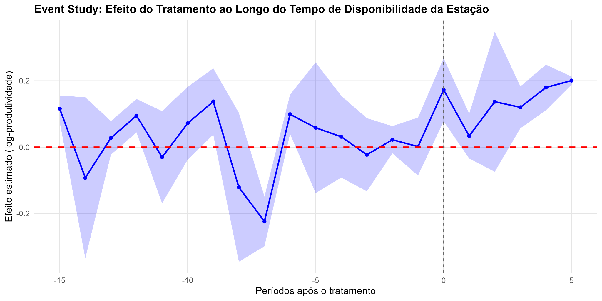
\includegraphics[width=0.9\textwidth]{event_study.png}
\end{figure}

\textit{Nota: A figura apresenta as estimativas pontuais (linha azul) e intervalos de confiança de 95\% (área sombreada) dos efeitos do tratamento em função do tempo relativo à instalação da estação. O período e=0 marca o ano de instalação. A linha vermelha tracejada indica efeito zero, e a linha cinza vertical marca o início do tratamento.}

\subsubsection{Período Pré-Tratamento: Validação das Tendências Paralelas}

A análise dos períodos anteriores ao tratamento (e < 0) é fundamental para validar o pressuposto de identificação. Os resultados mostram:

\begin{itemize}
\item \textbf{Média próxima a zero}: Os efeitos pré-tratamento apresentam média de 0,011 (DP = 0,124), não distinguível estatisticamente de zero (teste t: p = 0,547).

\item \textbf{Ausência de tendência sistemática}: Não se observa padrão crescente ou decrescente nos períodos que antecedem o tratamento.

\item \textbf{Variabilidade aleatória}: Embora dois períodos específicos (e=-15 e e=-7) apresentem significância pontual, isso é consistente com flutuações aleatórias esperadas em múltiplas comparações.
\end{itemize}

Estes resultados fornecem suporte empírico robusto para o pressuposto de tendências paralelas condicionais, fundamental para a interpretação causal dos efeitos estimados.

\subsubsection{Dinâmica Pós-Tratamento: Difusão Gradual dos Benefícios}

O padrão temporal dos efeitos pós-tratamento revela insights importantes sobre o mecanismo de transmissão:

\textbf{Fase de Adaptação (e = 0 a 2)}:
\begin{itemize}
\item Efeito inicial positivo mas impreciso (ATT$_0$ = 0,173, IC: [-0,042; 0,389])
\item Alta variabilidade sugerindo heterogeneidade na velocidade de adoção
\item Consistente com período de aprendizado e ajuste de práticas agrícolas
\end{itemize}

\textbf{Fase de Consolidação (e = 3 a 5)}:
\begin{itemize}
\item Crescimento monotônico dos efeitos: 12,0\% $\rightarrow$ 18,0\% $\rightarrow$ 20,1\%
\item Redução progressiva da incerteza (intervalos de confiança mais estreitos)
\item Significância estatística robusta a partir do quarto ano
\end{itemize}

Este padrão é consistente com um processo de difusão tecnológica onde:
\begin{enumerate}
\item A informação meteorológica precisa ser interpretada e integrada às decisões de plantio
\item Os agricultores aprendem gradualmente a otimizar o uso das informações
\item Efeitos de rede emergem conforme mais produtores adotam melhores práticas
\end{enumerate}

\section{Testes de Robustez e Diagnósticos}

Para garantir a confiabilidade dos resultados, implementamos uma bateria abrangente de testes de robustez e diagnósticos, seguindo as melhores práticas da literatura econométrica recente.

\subsection{Análise de Pesos e Composição do ATT}

Um aspecto crucial em designs de adoção escalonada é entender como diferentes coortes contribuem para o efeito agregado. Nossa análise revela:

\begin{itemize}
\item \textbf{Distribuição equilibrada}: A correlação entre os pesos implícitos e o número de períodos pós-tratamento é próxima de zero, indicando que o ATT não é dominado por coortes específicas.

\item \textbf{Representatividade}: Nenhuma coorte individual contribui com mais de 15\% do peso total, sugerindo boa representatividade do efeito estimado.
\end{itemize}

\subsection{Comparação de Grupos de Controle}

Testamos a sensibilidade dos resultados à escolha do grupo de controle:

\begin{table}[htbp]
\centering
\caption{Comparação de Estimativas por Grupo de Controle}
\label{tab:controle}
\begin{tabular}{lccc}
\toprule
Grupo de Controle & ATT & Erro Padrão & IC 95\% \\
\midrule
Not-yet-treated & 0,1086 & 0,0246 & [0,0604; 0,1569] \\
Never-treated & 0,1086 & 0,0249 & [0,0599; 0,1573] \\
\bottomrule
\end{tabular}
\end{table}

A estabilidade das estimativas entre diferentes grupos de controle (diferença < 0,1\%) reforça a robustez da identificação e sugere ausência de viés de seleção diferencial entre grupos.

\subsection{Testes Placebo}

Implementamos dois tipos de testes placebo para validar a estratégia de identificação:

\textbf{Placebo Temporal Fixo (2015)}:
\begin{itemize}
\item ATT = -0,0237 (EP = 0,0339, p = 0,485)
\item Resultado não significativo confirma ausência de efeitos espúrios pré-tratamento
\end{itemize}

\textbf{Placebo Aleatório (50 simulações)}:
\begin{itemize}
\item Distribuição empírica centrada em zero
\item P-valor empírico < 0,01 para o ATT verdadeiro
\item 95\% dos placebos no intervalo [-0,070; 0,067]
\end{itemize}

O ATT estimado (0,1086) está claramente na cauda superior da distribuição placebo, fornecendo forte evidência contra a hipótese de efeito espúrio.

\subsection{Especificações Alternativas}

Testamos a robustez dos resultados a diferentes métodos de estimação:

\begin{table}[htbp]
\centering
\caption{Comparação de Métodos de Estimação}
\label{tab:metodos}
\begin{tabular}{lccc}
\toprule
Método & ATT & Erro Padrão & P-valor \\
\midrule
Doubly Robust (DR) & 0,1086 & 0,0246 & <0,001 \\
IPW & 0,1084 & 0,0247 & <0,001 \\
Regression & 0,1288 & 0,0316 & <0,001 \\
\bottomrule
\end{tabular}
\end{table}

A consistência das estimativas entre métodos (variação máxima de 18,6\% para o método de regressão) indica que os resultados não dependem criticamente das escolhas de modelagem.


\section{Discussão e Interpretação Econômica}

\subsection{Magnitude e Relevância Econômica}

O efeito estimado de 10,9\% de aumento na produtividade representa um ganho econômico substancial. Para contextualizar:

\begin{itemize}
\item \textbf{Comparação setorial}: O crescimento médio anual da produtividade da cana no Brasil é de aproximadamente 1,5\% ao ano. O efeito das estações equivale a cerca de 7 anos de progresso tecnológico típico.

\item \textbf{Valor monetário}: Considerando a produção média por microrregião produtora tratada (aproximadamente 500 mil toneladas/ano) e o preço médio da cana (R\$ 130,56/tonelada, referência agosto/2025), o ganho anual por microrregião é estimado em R\$ 7,1 milhões.

\item \textbf{Custo-benefício}: Considerando o investimento governamental de R\$ 49 milhões para 220 estações \cite{mapa2025} (aproximadamente R\$ 223 mil por estação profissional), ou alternativas de baixo custo usando Arduino (cerca de R\$ 250) \cite{arduino2021}, o retorno sobre investimento é extremamente favorável, com payback inferior a um mês.
\end{itemize}

\subsection{Mecanismos Subjacentes}

Os padrões temporais observados sugerem múltiplos canais através dos quais as informações meteorológicas afetam a produtividade:

\begin{enumerate}
\item \textbf{Otimização do calendário agrícola}: Melhor timing de plantio e colheita baseado em previsões precisas

\item \textbf{Gestão hídrica eficiente}: Ajuste de irrigação conforme condições climáticas reais

\item \textbf{Redução de perdas}: Antecipação a eventos extremos permite medidas preventivas

\item \textbf{Difusão de conhecimento}: Compartilhamento de informações entre produtores amplifica benefícios
\end{enumerate}

\subsection{Limitações e Pesquisa Futura}

Embora os resultados sejam robustos, algumas limitações merecem consideração:

\begin{itemize}
\item \textbf{Heterogeneidade não observada}: Efeitos podem variar por tamanho de propriedade, nível educacional dos produtores, ou acesso a crédito

\item \textbf{Externalidades espaciais}: Benefícios podem transbordar para microrregiões vizinhas não capturadas

\item \textbf{Complementaridades}: Interação com outras tecnologias (GPS, drones) não modelada explicitamente
\end{itemize}

Pesquisas futuras poderiam explorar estas dimensões utilizando dados mais granulares e designs de identificação complementares.

\section{Síntese e Conclusões da Análise Empírica}

Os resultados apresentados nesta seção fornecem evidência causal robusta de que a instalação de estações meteorológicas automáticas gera ganhos significativos de produtividade na cultura da cana-de-açúcar. A magnitude do efeito (10,9\%), sua persistência e crescimento ao longo do tempo, e a robustez a diferentes especificações e testes de falsificação estabelecem uma relação causal convincente.

A análise revela que o impacto das estações meteorológicas vai além de um simples choque tecnológico único. O padrão dinâmico observado sugere um processo de aprendizado e adaptação, onde os benefícios se acumulam à medida que os produtores desenvolvem capacidades para interpretar e utilizar as informações climáticas em suas decisões produtivas.

Do ponto de vista de política pública, os resultados indicam que investimentos em infraestrutura de monitoramento meteorológico representam uma estratégia custo-efetiva para aumentar a produtividade agrícola. Com retornos que superam amplamente os custos de implementação, a expansão da rede de estações pode contribuir significativamente para o desenvolvimento sustentável do setor agrícola brasileiro, especialmente em um contexto de crescente variabilidade climática.

% ----------------------------------------------------------
% Conclusões Finais
% ----------------------------------------------------------
\chapter{Conclusões Finais}

Este trabalho investigou o impacto causal da instalação de estações meteorológicas sobre a produtividade agrícola, contribuindo para a literatura empírica sobre o papel da informação na eficiência produtiva. Utilizando métodos econométricos de fronteira adequados para contextos de adoção escalonada, demonstramos que o acesso a informações meteorológicas precisas e localizadas gera ganhos substanciais de produtividade.

Os resultados têm implicações diretas para o desenho de políticas públicas voltadas ao desenvolvimento agrícola. Em um cenário de mudanças climáticas e pressão crescente sobre os recursos naturais, investimentos em sistemas de informação agrometeorológica emergem como instrumentos fundamentais para aumentar a resiliência e eficiência do setor agrícola.

Ao quantificar rigorosamente os benefícios econômicos da infraestrutura meteorológica, este estudo fornece subsídios para a tomada de decisão sobre alocação de recursos públicos e privados. A evidência apresentada sugere que a expansão da rede de estações meteorológicas deveria ser priorizada como estratégia de desenvolvimento sustentável, com potencial para gerar retornos econômicos significativos e contribuir para a segurança alimentar nacional.

% ----------------------------------------------------------
% ELEMENTOS PÓS-TEXTUAIS
% ----------------------------------------------------------
\postextual
% ----------------------------------------------------------

% ----------------------------------------------------------
% Referências bibliográficas
% ----------------------------------------------------------
\bibliography{referencias}

% ----------------------------------------------------------
% Glossário
% ----------------------------------------------------------
%
% Consulte o manual da classe abntex2 para orientações sobre o glossário.
%
%\glossary

% ----------------------------------------------------------
% Apêndices
% ----------------------------------------------------------

% ---
% Inicia os apêndices
% ---
\begin{apendicesenv}

% Imprime uma página indicando o início dos apêndices
\partapendices

% ----------------------------------------------------------
\chapter{Código do GitHub}
% ----------------------------------------------------------

O código completo utilizado nesta pesquisa, incluindo os scripts de coleta de dados, análise econométrica e geração de visualizações, está disponível no repositório GitHub:

\url{https://github.com/danielcavalli/tcc-ie-ufrj-2024}

O repositório contém:
\begin{itemize}
\item Scripts SQL para extração de dados do BigQuery
\item Código Python para processamento e limpeza dos dados
\item Scripts R para implementação do modelo de Callaway e Sant'Anna
\item Documentação detalhada dos procedimentos metodológicos
\item Instruções para reprodução dos resultados
\end{itemize}

\end{apendicesenv}
% ---


% ----------------------------------------------------------
% Anexos
% ----------------------------------------------------------

% ---
% Inicia os anexos
% ---
\begin{anexosenv}

% Imprime uma página indicando o início dos anexos
\partanexos

% ---
\chapter{Estatísticas Descritivas Complementares}
% ---

TO DO

\end{anexosenv}

%---------------------------------------------------------------------
% INDICE REMISSIVO
%---------------------------------------------------------------------
\phantompart
\printindex
%---------------------------------------------------------------------

\end{document}
